\section{Zustandsraumdarstellung (ZRD)}

\textbf{Grundidee:} Differentialgleichung $n.$ Ordnung eines Systems durch ein \textbf{Differentialgleichungssystem} 
von $n$ Gleichungen $1.$ Ordnung darzustellen.


\subsection{Vorteile der ZRD}{253-254}
\begin{itemize}
    \item Innere Systemstabilitäten können erkannt werden, die bei der Untersuchung der UTF 
        nicht festgestellt werden können \textrightarrow\ Einblick in den \textbf{inneren Aufbau} eines Systems
    \item Wichtig in der Regelungstechnik
    \item ZRD hat Vorteile bei der \textbf{numerischen} Behandlung von Systemen
    \item Beschreibung durch \textbf{Energiespeicher}, in der Elektrotechnik L und C
    \item \textbf{Nur Integratoren} werden verwendet, keine Differentiatoren
\end{itemize}


\subsection{Zustandsraumdarstellung (ZRD) im Zeitbereich}{255}
\label{ZRD Zeitbereich}

\begin{minipage}[c]{0.4\columnwidth}
    \vspace{-0.3cm}
    
    \begin{empheq}[box=\fbox] {align*}
        \underline{\dot{x}}(t) &= \bm{A} \underline{x}(t) + \bm{B} \underline{u}(t) \\
        \underline{y}(t) &= \bm{C} \underline{x}(t) + \bm{D} \underline{u}(t)
    \end{empheq}

    \begin{tabular}{ll@{}}
        $\underline{u}(t)$   & Eingangsvektor ($m$ Zeilen) \\
        $\underline{x}(t)$   & Zustandsvektor ($n$ Zeilen) \\
        $\underline{y}(t)$   & Ausgangsvektor ($k$ Zeilen) \\
    \end{tabular}

\end{minipage}
\hfill
\begin{minipage}[c]{0.58\columnwidth}
    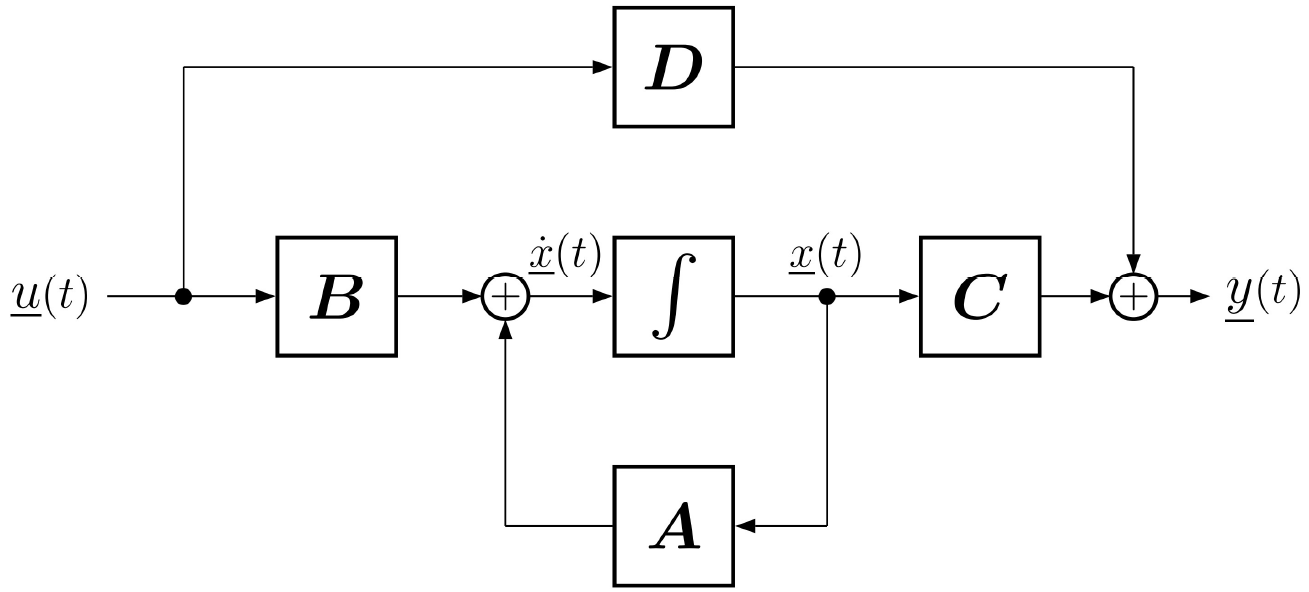
\includegraphics[width=\columnwidth]{images/blockdiagramm_zustandsdarstellung.png}
\end{minipage}


\begin{itemize}
    \item obere Gleichung: \textbf{Zustandsgleichung}
    \item untere Gleichung: \textbf{Ausgangsgleichung}
    \item $\bm{A}$ \textbf{Systemmatrix} ($n \times n$-Matrix) \\
        Sie bestimmt das Verhalten des \textbf{ungestörten Systems} ($\underline{u}(t) = 0$)
        und bestimmt z.B. die innere Stabilität des gesamten Systems.
    \item $\bm{B}$ \textbf{Eingangsmatrix (Steuermatrix)} ($n \times m$-Matrix) \\
        Sie bestimmt die Wirkung der \textbf{Steuergrössen} $\underline{u}(t)$ auf die \textbf{Zustandsgrössen} $\underline{x}(t)$
    \item $\bm{C}$ \textbf{Ausgangsmatrix (Beobachtungsmatrix)} ($k \times n$-Matrix) \\
        Sie kennzeichnet die Abhängigkeit des \textbf{Zustandes} $\underline{x}(t)$ von der beobachtbaren Ausgangsgrösse $\underline{y}(t)$
    \item $\bm{D}$ \textbf{Durchgangsmatrix} ($k \times m$-Matrix) \\
        Sie bestimmt die unmittelbare Wirkung der Eingangsgrösse $\underline{u}(t)$ auf den Ausgang $\underline{y}(t)$
\end{itemize}


\example{ZRD aus Schaltung aufstellen}

\begin{minipage}[c]{0.48\columnwidth}
    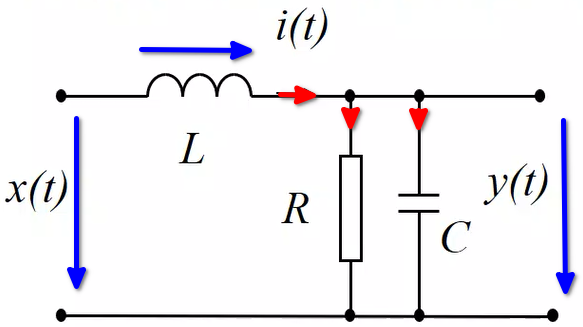
\includegraphics[width=0.9\columnwidth]{images/beispiel_zrd_aus_schaltung.png}
\end{minipage}
\hfill
\begin{minipage}[c]{0.48\columnwidth}
    \begin{itemize}
        \item DGL Induktivität: $\frac{\diff i_L(t)}{\diff t} = \frac{u_L(t)}{L}$ \\
            \textrightarrow\ $u_L(t) = L \cdot \frac{\diff i_L(t)}{\diff t}$
        \item DGL Kapazität: $\frac{\diff u_C(t)}{\diff t} = \frac{i_C(t)}{C}$ \\
        \textrightarrow\ $u_C(t) = \frac{1}{C} \int\limits_{- \infty}^t i(\tau) \, \diff \tau$
    \end{itemize}
\end{minipage}

\begin{minipage}[c]{0.5\columnwidth}
    \begin{empheq}[box=\fbox] {align*}
        \text{Maschen: } & L \cdot \frac{\partial i(t)}{\partial t} + y(t) = x(t) \\
        \text{Knoten: }  & \frac{1}{C} \int\limits_{- \infty}^t \Big( i(\tau) - \frac{y(\tau)}{R} \Big) \, \diff \tau = y(t)
    \end{empheq}
\end{minipage}
\hfill
\begin{minipage}[c]{0.48\columnwidth}
    Beide Gleichungen in ihre differentielle Form bringen (zweite Gleichung ableiten)
\end{minipage}

\begin{minipage}[c]{0.5\columnwidth}
    \begin{align*}
        L \cdot i'(t) + y(t) &= x(t) \\
        i(t) - \frac{y}{R} &= C \cdot y'(t) 
    \end{align*}
\end{minipage}
\hfill
\begin{minipage}[c]{0.48\columnwidth}
    Gleichungen umformen, sodass die ZRD aufgestellt werden kann
\end{minipage}

\begin{minipage}[c]{0.5\columnwidth}
    \begin{align*}
        i'(t) &= - \frac{1}{L} y(t) + \frac{1}{L} x(t) \\
        y'(t) &= \frac{1}{C} i(t) - \frac{1}{RC} y(t) 
    \end{align*}
\end{minipage}
\hfill
\begin{minipage}[c]{0.48\columnwidth}
    \begin{tabular}{ll}
        Zustände:   & $i(t)$, $y(t)$ \\
        Eingang:    & $x(t)$ \\
        Ausgang:    & $\tilde{y}(t) = y(t)$ \\
    \end{tabular}
    
    % \textrightarrow\ Gleichungssystem in Matrixform schreiben
\end{minipage}

\begin{empheq}[box=\fbox] {align*}
    \begin{bmatrix} i'(t) \\ y'(t) \end{bmatrix} &= \underbrace{ \begin{bmatrix} 0 & -\frac{1}{L} \\ \frac{1}{C} & -\frac{1}{RC} \end{bmatrix} }_{\bm{A}}
    \cdot \begin{bmatrix} i(t) \\ y(t) \end{bmatrix} + \underbrace{ \begin{bmatrix} \frac{1}{L} \\ 0 \end{bmatrix} }_{\bm{B}} \cdot x(t) \\
    \tilde{y}(t) &= \underbrace{ \begin{bmatrix} 0 & 1 \end{bmatrix}}_{\bm{C}} \cdot \begin{bmatrix} i(t) \\ y(t) \end{bmatrix} + \underbrace{ \begin{bmatrix} 0 \end{bmatrix} }_{\bm{D}} \cdot x(t)
\end{empheq}


\example{ZRD aus Signalflussdiagramm aufstellen}

Das ZRD zu folgendem System soll aufgestellt werden. Dazu müssen die Matritzen $\bm{A}, \bm{B}, \bm{C}$ und $\bm{D}$ gefunden werden.
$$ \text{Zustandsvektor: }  \underline{q}(t) =  \begin{pmatrix} q_1(t) \\ q_2(t) \\ q_3(t) \end{pmatrix} 
\text{ und dessen Ableitung } \underline{\dot{q}}(t) = \begin{pmatrix} \dot{q}_1(t) \\ \dot{q}_2(t) \\ \dot{q}_3(t) \end{pmatrix} $$
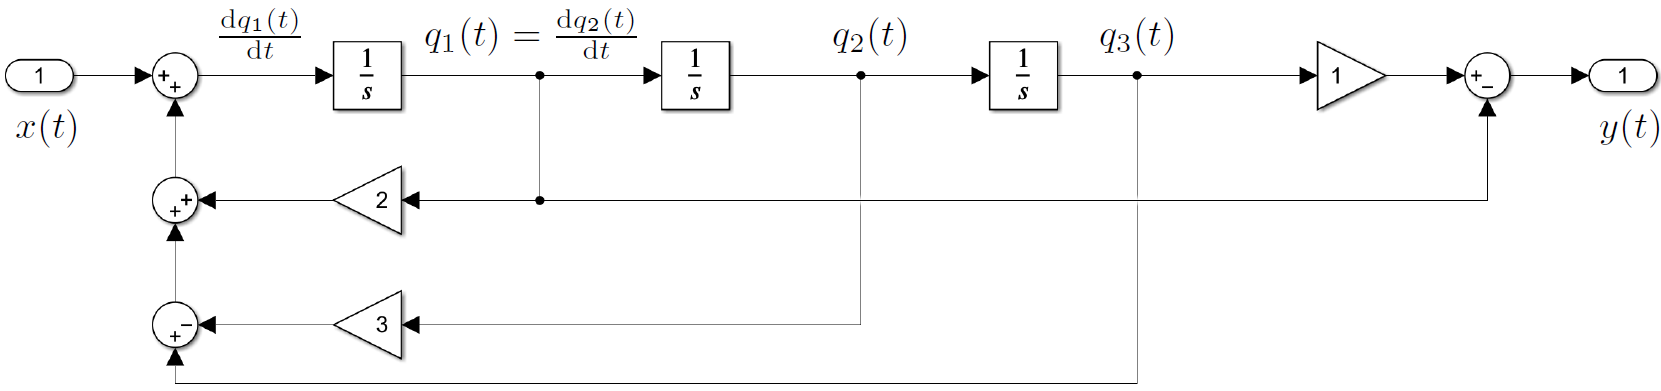
\includegraphics[width=\columnwidth]{images/beispiel_zrd_aus_sfd.png}

\begin{empheq}[box=\fbox] {align*}
    \underbrace{ \begin{pmatrix} \dot{q}_1(t) \\ \dot{q}_2(t) \\ \dot{q}_3(t) \end{pmatrix} }_{\underline{\dot{q}}(t)} &= 
    \underbrace{ \begin{bmatrix} 2 & -3 & 1 \\ 1 & 0 & 0 \\ 0 & 1 & 0 \end{bmatrix} }_{\bm{A}}
    \cdot \underbrace{ \begin{pmatrix} q_1(t) \\ q_2(t) \\ q_3(t) \end{pmatrix} }_{\underline{q}(t)} 
    + \underbrace{ \begin{bmatrix} 1 \\ 0 \\ 0 \end{bmatrix} }_{\bm{B}} \cdot x(t) \\
    y(t) &= \underbrace{ \begin{bmatrix} -1 & 0 & 1 \end{bmatrix}}_{\bm{C}} 
    \cdot \underbrace{ \begin{pmatrix} q_1(t) \\ q_2(t) \\ q_3(t) \end{pmatrix} }_{\underline{q}(t)} 
    + \underbrace{ \begin{bmatrix} 0 \end{bmatrix} }_{\bm{D}} \cdot x(t)
\end{empheq}


\subsection{Zustandsraumdarstellung (ZRD) im Laplace-Bereich}{264}

\begin{minipage}[c]{0.44\columnwidth}
    \vspace{-0.3cm}
    
    \begin{empheq}[box=\fbox] {align*}
        s \underline{X}(s) - x(0) &= \bm{A} \underline{X}(s) + \bm{B} \underline{U}(s) \\
        \underline{Y}(s) &= \bm{C} \underline{X}(s) + \bm{D} \underline{U}(s)
    \end{empheq}

    \begin{tabular}{ll@{}}
        $\underline{U}(s)$   & Eingangsvektor ($m$ Zeilen) \\
        $\underline{X}(s)$   & Zustandsvektor ($n$ Zeilen) \\
        $\underline{Y}(s)$   & Ausgangsvektor ($k$ Zeilen) \\
        $\bm{I}$             & Einheitsmatrix \\
        $\bm{H(s)}$          & Übertragungsmatrix ($k \times m$)\\
    \end{tabular}

\end{minipage}
\hfill
\begin{minipage}[c]{0.54\columnwidth}
    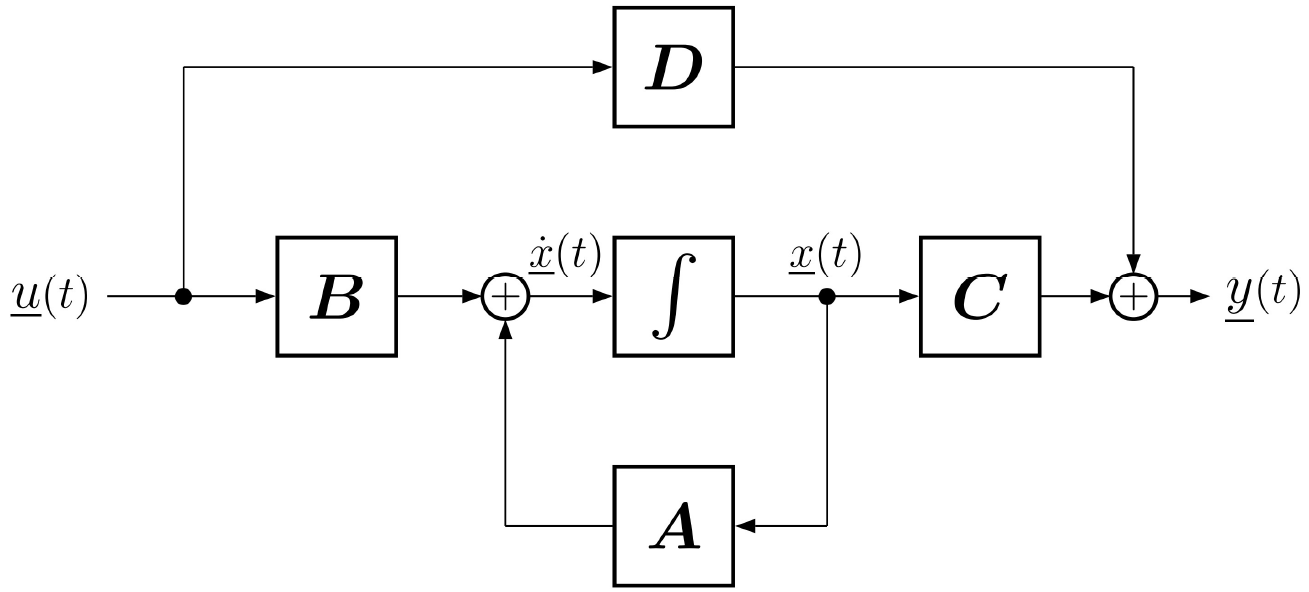
\includegraphics[width=\columnwidth]{images/blockdiagramm_zustandsdarstellung.png}
\end{minipage}

\vspace{0.2cm}
$$ \boxed{ \underline{Y}(s) = \bm{C}(s \bm{I} - \bm{A})^{-1} \underline{x}(0) 
    + \underbrace{(\bm{C}(s \bm{I} - \bm{A})^{-1} \bm{B} + \bm{D} )}_{\bm{H(s)}} \underline{U}(s) } $$

Mit Anfangsbedingungen $x(0) = 0$ ergibt sich folgender Zusammenhang, was der Übertragungsfunktion (UTF) entspricht,
aber im allgemeinen Fall eine \textbf{Matrix} ist.
$$ \boxed{ \underline{Y}(s) = \underbrace{(\bm{C}(s \bm{I} - \bm{A})^{-1} \bm{B} + \bm{D} )}_{\bm{H(s)}} \underline{U}(s) } $$

\textbf{Hinweis:} Aus einem Signalflussdiagramm (SFD) ist es meist sehr einfach, die gesuchten Grössen der ZRD zu finden.


\subsubsection{Übertragungsmatrix und Übertragungsfunktion}{266}

\begin{minipage}[t]{0.48\columnwidth}
    \begin{center}
        \textbf{\myul{Übertragungsmatrix}}
    \end{center}
    \begin{itemize}
        \item MIMO-Systeme
        \item Beschreibung in Matritzenform
            $$ Y(s) = \bm{H(s)} \cdot U(s) $$
        \item  $H(s)$ hat gleiche Grösse (Dimensionen) wie Durchgangsmatrix $\bm{D}$
    \end{itemize}
\end{minipage}
\hfill
\begin{minipage}[t]{0.48\columnwidth}
    \begin{center}
        \textbf{\myul{Übertragungsfunktion}}
    \end{center}
        \begin{itemize}
            \item SISO-Systeme
            \item Matrix-Form wird zu 'normaler' Gleichung
            $$ Y(s) = H(s) \cdot U(s) $$
        \end{itemize}
\end{minipage}


\subsection{Ordnung eines Systems}{256}

Die \textbf{Ordnung} eines Systems definiert die \textbf{kleinste Anzahl von Zustandsgrössen} $x(t)$.
Äquivalent dazu kann die Ordnung eines Systems auch als die \textbf{Anzahl der unabhängigen Energiespeicher} definiert werden.


\subsection{ZRD mit Matlab}

$$ H(s) = \frac{b_i s^i + b_{i-1} s^{i-1} \cdots b_1 s^1 + b_0}{a_i s^i + a_{i-1} s^{i-1} \cdots a_1 s^1 + a_0} $$
\lstinputlisting{snippets/zrd_frequenzbereich.m}


\subsection{Äquivalente Zustandsraumdarstellung (ZRD)}{257}

Mit einer \textbf{Transformationsmatrix} $\bm{T}$ ($n \times n$-Matrix, nicht singulär, $\bm{T T^{-1} = I = T^{-1} T}$) kann man 
\textbf{verschiedenste Zustandsgrössen und Zustandsraumdarstellungen} erhalten, die aber alle ein 
\textbf{identisches Systemverhalten} aufweisen. \\
% Somit kann eine ZRD durch \textbf{verschiedene Schaltungen} realisiert werden, solange diese Schaltungen die 
% \textbf{gleiche Übertragungsfunktion} liefern!


% TODO
\begin{minipage}[c]{0.4\columnwidth}
    \vspace{-0.3cm}
    
    \begin{empheq}[box=\fbox] {align*}
        \underline{\dot{\xi}}(t) &= \overbrace{ \bm{ T A T}^{-1}}^{\bm{\hat{A}}} \underline{\xi}(t) + \overbrace{\bm{T B}}^{\bm{\hat{B}}}  \underline{u}(t) \\
        \underline{y}(t) &= \underbrace{\bm{C T}^{-1}}_{\bm{\hat{C}}} \underline{\xi}(t) + \underbrace{\bm{D}}_{\bm{\hat{D}}} \underline{u}(t)
    \end{empheq}
    % \begin{tabular}{ll}
    %     Zusammenhänge 
    % \end{tabular}

\end{minipage}
\hfill
\begin{minipage}[c]{0.58\columnwidth}
    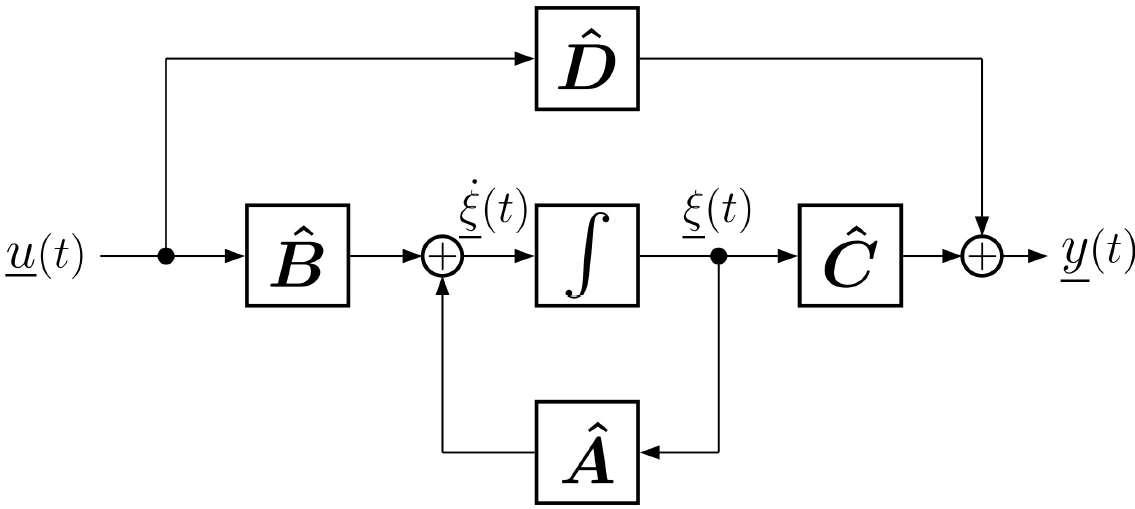
\includegraphics[width=\columnwidth]{images/aequivalente_zrd.png}
\end{minipage}

Die obige ZRD ist \textbf{äquivalent} zur ZRD aus Abschnitt ~\ref{ZRD Zeitbereich} bezüglich $\underline{y}(t)$ und $\underline{u}(t)$.
Die bedeutet, dass die \textbf{Zustandsgrössen} $\underline{\xi}(t)$ und $\underline{x}(t)$ \textbf{willkürlich} gewählt 
werden können, solange $\bm{T}$ nicht singulär ist (Determinante von $\bm{T} \neq 0$) \\

Physikalisch sinnvolle Zustandsgrössen sind:
\begin{itemize}
    \item Spannungen über Kapazitäten
    \item Ströme durch Induktivitäten
\end{itemize}


% \subsubsection{Bedingungen für Äquivalenz}  % TODO

% % blaue Schrift auf V8, F19? -> gilt für dieses Beispiel
% \begin{itemize}
%     \item bla
% \end{itemize}



\subsection[Matrix bm{A} diagonalisieren]{Matrix $\bm{A}$ diagonalisieren}

Oft wird die \textbf{Systemmatrix} $\bm{A}$ diagonalisiert, um \textbf{entkoppelte Zustände} zu erhalten. Anstelle der Matrix
$\bm{\hat{A}} = \bm{ T A T}^{-1}$ wird dann üblicherweise $\bm{A_{diag}}$ verwenet.

\begin{tabular}{ll}
    $\lambda_i$                     & Eigenwerte der Matrix $\bm{A}$ \\
    $\vec{v}_i$                     & Eigenvektoren der Matrix $\bm{A}$ \\
    $\bm{V}$                        & Matrix mit Eigenvektoren von $\bm{A}$ \\
    $\bm{A_{diag}} = \bm{\Lambda}$  & Diagonalisierte Matix $\bm{A}$ mit Eigenwerten $\lambda_i$ auf Diagonale \\
    $\bm{T}$                        & Transformationsmatrix 
\end{tabular}

\begin{minipage}[c]{0.48\columnwidth}
    $$ \boxed{\bm{A_{diag}} = \bm{\Lambda} =  \bm{V}^{-1} \cdot \bm{A} \cdot \bm V} $$
\end{minipage}
\hfill
\begin{minipage}[c]{0.48\columnwidth}
    \begin{empheq}[box=\fbox] {align*}
        \bm{T} &= \bm{V}^{-1} \\
        \bm{T}^{-1} &= \bm{V} 
    \end{empheq}
\end{minipage}


\subsubsection{Vorgehen Matrix diagonalisieren}

\begin{outline}
    \1 Ansatz: $ \bm{A} \cdot \vec{v} = \lambda \cdot \vec{v}$ \textrightarrow\ $(\bm{A} - \lambda \bm{I}) \cdot \vec{v} = \vec{0}$ bzw. 
        $(\lambda \bm{I} - \bm{A}) \cdot \vec{v} = \vec{0}$
    \1 Determinante des charakteristischen Polynoms Null setzen: $\abs{\lambda \bm{I} - \bm{A}} = 0$ \\
        \textrightarrow\ Eigenwerte $\lambda_i$ 
    \1 Für jeden gefundenen Eigenwert müssen Eigenvektoren $\vec{v}_i$ gefunden werden:
        \2 Eigenwert $\lambda_i$ in Gleichungssystem $(\lambda_i \bm{I} - \bm{A}) \cdot \vec{v}_i = \vec{0}$ einsetzen
        \2 Einen Wert von $\vec{v}_i = 1$ wählen und Eigenvektor $\vec{v}_i$ als Spaltenvektor schreiben
    \1 Matrix $\bm{V}$ aus Eigenvektoren 'zusammenbauen'
    \1 Matrix $\bm{\Lambda}$ 'zusammenbauen', indem man Eigenwerte $\lambda_i$ auf Diagonale schreibt
\end{outline}


\subsubsection{Entkoppeltes vs. nicht-entkoppeltes System}

\begin{minipage}[t]{0.4\columnwidth}
    \begin{center}
        \myul{\textbf{Nicht-entkoppeltes System}}
    \end{center}
    $$ \bm{A} = \begin{bmatrix*}[r] -2 & 7 \\ -1 & 6 \end{bmatrix*} $$
    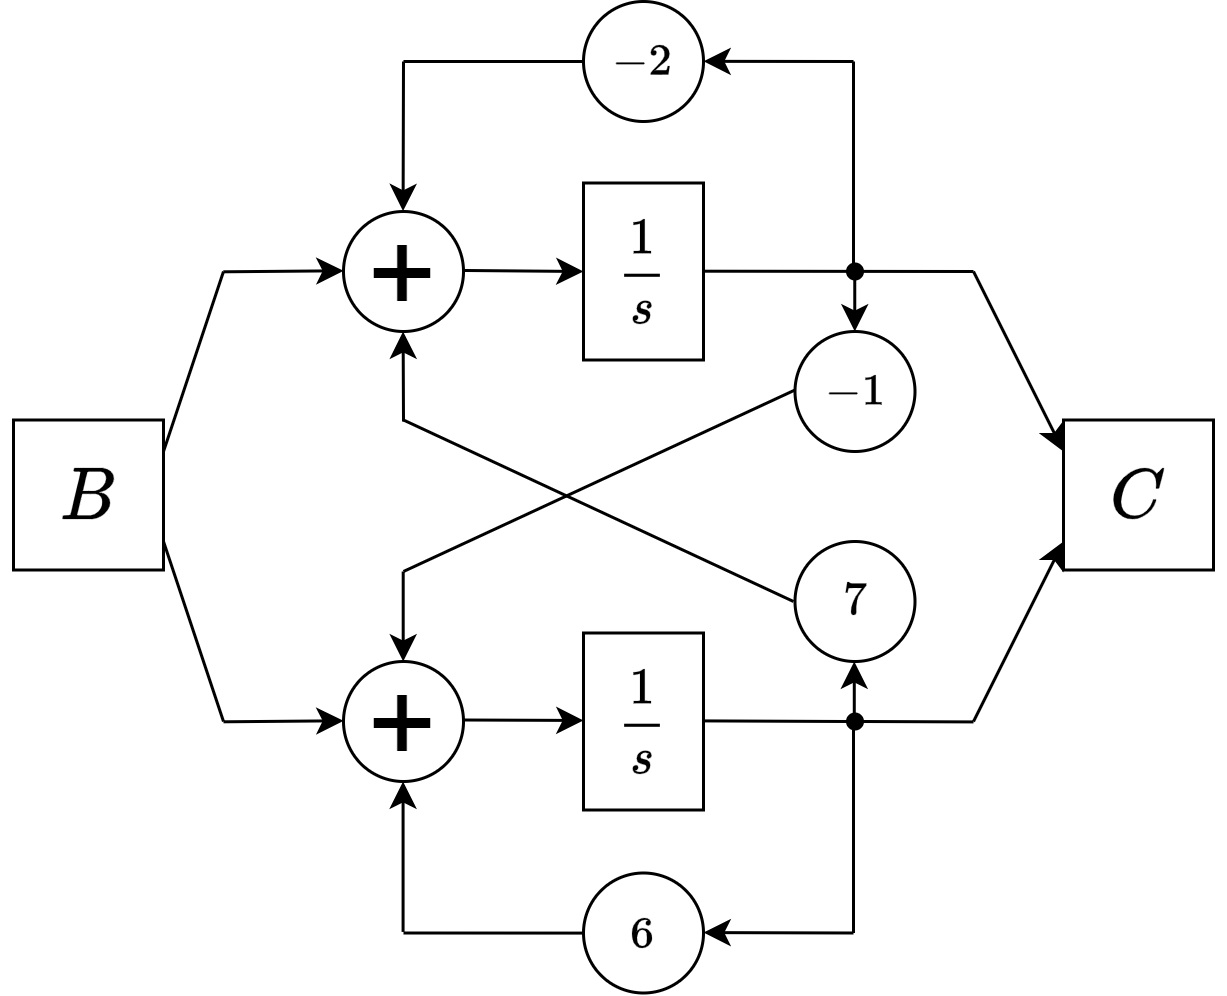
\includegraphics[width=\columnwidth]{images/kreuzform.png}
\end{minipage}
\hfill
\begin{minipage}[t]{0.48\columnwidth}
    \begin{center}
        \myul{\textbf{Entkoppeltes System}}
    \end{center}
    $$ \bm{A_{diag}} = \begin{bmatrix*}[r] -1 & 0 \\ 0 & 5 \end{bmatrix*} $$
    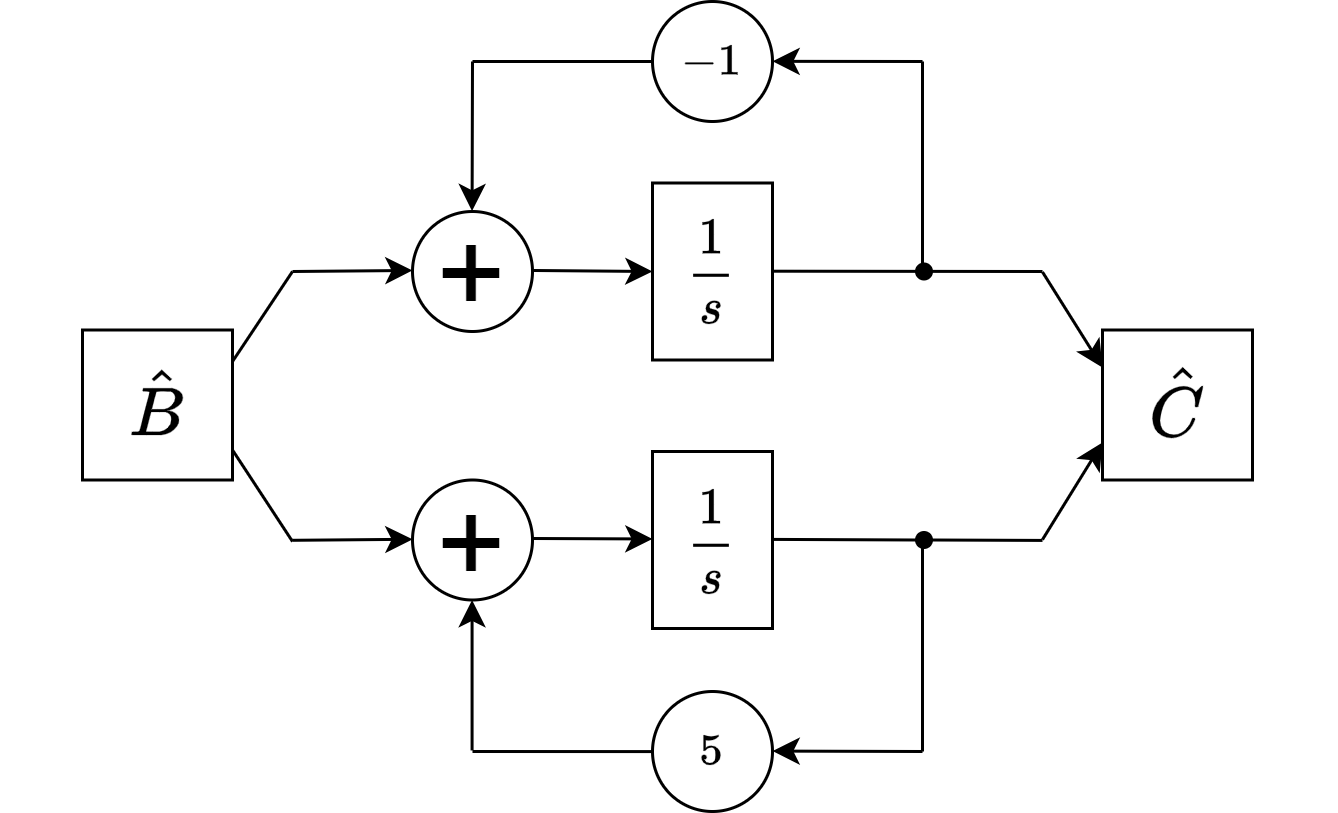
\includegraphics[width=\columnwidth]{images/parallelform.png}
\end{minipage}


\subsection{Einschub -- Lineare Algebra: 2x2 Matrix invertieren}

\begin{minipage}[b]{0.33\columnwidth}
    $$ \bm{A} = 
    \begin{bmatrix*}[r]
        a & b \\
        c & d 
    \end{bmatrix*} $$
\end{minipage}
\hfill
\begin{minipage}[b]{0.66\columnwidth}
    $$ \bm{A}^{-1} = \frac{1}{\det(\bm{A})} \cdot 
    \begin{bmatrix*}[r]
        d & -b \\
        -c & a 
    \end{bmatrix*} \quad \text{ mit } \det(\bm{A}) = ad - bc $$
\end{minipage}


\example{Matrix-Diagonalisierung}{258}

\begin{minipage}[c]{0.25\columnwidth}
    $$ \bm{A} = \begin{bmatrix*}[r]
        -2 & 7 \\
        -1 & 6 
    \end{bmatrix*}$$ 
\end{minipage}
\hfill
\begin{minipage}[c]{0.72\columnwidth}
    $$ \abs{\lambda \bm{I} - \bm{A}} = \begin{vmatrix*}[c]
        \lambda + 2 & -7 \\
        1 & \lambda - 6 
    \end{vmatrix*} = (\lambda + 2) \cdot (\lambda - 6) - 7 \cdot (-1) = 0 $$
\end{minipage}

\textrightarrow\ Mitternachtsformel liefert die Eigenwerte $\lambda_1 = -1$ und $\lambda_2 = 5$

\begin{minipage}[t]{0.56\columnwidth}
    Ersten Eigenwert $\lambda_1 = -1$ in $(\lambda_1 \bm{I} - \bm{A}) \cdot \vec{v}_1 = \vec{0}$ einsetzen
\end{minipage}
\hfill
\begin{minipage}[c]{0.4\columnwidth}
    \begin{align*}
        1 \cdot v_{11} - 7 \cdot v_{21} &= 0 \\
        1 \cdot v_{11} - 7 \cdot v_{21} &= 0 
    \end{align*}
\end{minipage}

\begin{minipage}[c]{0.4\columnwidth}
    Wähle $v_{21} = 1$ \quad \textrightarrow\ $ \vec{v}_1 = \begin{bmatrix*}[r] 7 \\ 1 \end{bmatrix*} $
\end{minipage}
\hfill
\begin{minipage}[c]{0.56\columnwidth}
   Gleichen Vorgehen für zweiten Eigenvektor $\vec{v}_2$
\end{minipage}

\begin{minipage}[c]{0.48\columnwidth}
    $$ \Lambda = \begin{bmatrix} \lambda_1 & 0 \\ 0 & \lambda_2 \end{bmatrix} $$
\end{minipage}
\hfill
\begin{minipage}[c]{0.48\columnwidth}
    $$ \bm{V} = \begin{bmatrix} \vec{v}_1 & \vec{v}_2 \end{bmatrix} = \begin{bmatrix} v_{11} & v_{12} \\ v_{21} & v_{22} \end{bmatrix} $$
\end{minipage}







